\documentclass[12pt, a4paper]{article}

\usepackage{import}
\usepackage{standalone}

\usepackage[top=4cm, right=2cm, bottom=2.7cm, left=2cm]{geometry}

\usepackage{wrapfig}
\usepackage{tabulary}
\usepackage{float}
\usepackage{pifont}
\usepackage{background}
\usepackage{tikz}


\pagestyle{empty}
\setlength{\parindent}{0pt}


\begin{document}
	
	\def\Arrow{{\scalebox{4}{$\Rightarrow$}}}
	\def\Image#1{\raisebox{-.5\height}{\includegraphics[width=3cm]{#1}}}
	
	\begin{minipage}{\textwidth}
		\section{Landschap \hfill\small Bron: Bebras}

			
			Onze bever volgt tekenles. De tekenleraar heeft hem een aantal opdrachten gegeven die hij in volgorde moet uitvoeren:
			\begin{enumerate}
				\item Teken wolken op de volledige onderste helft van een blad papier.
				\item Draai het blad een halve slag.
				\item Teken gras op de volledige onderste helft van het blad.
				\item Teken de zon bovenaan rechts op het blad papier.
			\end{enumerate}
			Als je deze opdrachten in de volgorde 1, 2, 3, 4 uitvoert, krijg je de volgende stappen:

			\begin{figure}[H]
				\flushleft
				\raisebox{-.5\height}{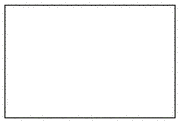
\includegraphics[width=0.27\linewidth]{image1}}
				\raisebox{-.5\height}{$\xrightarrow{(1)}$}
				\raisebox{-.5\height}{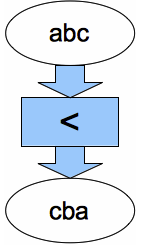
\includegraphics[width=0.27\linewidth]{image2}}
				\raisebox{-.5\height}{$\xrightarrow{(2)}$}
				\raisebox{-.5\height}{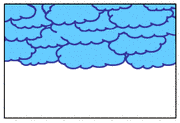
\includegraphics[width=0.27\linewidth]{image3}}
				\raisebox{-.5\height}{$\xrightarrow{(3)}$}
				\raisebox{-.5\height}{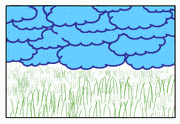
\includegraphics[width=0.27\linewidth]{image4}}
				\raisebox{-.5\height}{$\xrightarrow{(4)}$}
				\raisebox{-.5\height}{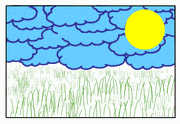
\includegraphics[width=0.27\linewidth]{image5}}
			\end{figure}
			
			Onze bever heeft de opdrachten goed begrepen, maar jammergenoeg vergist hij zich in de volgorde. Hij voert de opdrachten in de plaats uit \textbf{in de volgorde 3, 1, 2, 4}. Hoe zal zijn tekening er op het einde uitzien?
			
			\begin{table}[H]
				\begin{tabulary}{\linewidth}{|C|C|C|C|}
					\hline
					\textbf{A} & \textbf{B} & \textbf{C} & \textbf{D} \\
					
\includegraphics[width=\linewidth]{option1} &
					
\includegraphics[width=\linewidth]{option2} &
					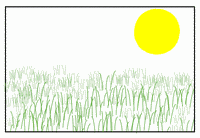
\includegraphics[width=\linewidth]{option3} &
					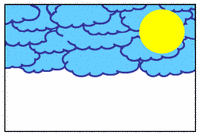
\includegraphics[width=\linewidth]{option4} \\
					\hline 
				\end{tabulary}
			\end{table}
	\end{minipage} \\ \\
	
\end{document}	